\chapter{Stage}
\label{ch:tesi:stage}

\section{Piano di stage}
\label{sec:tesi:stage:piano}

\subsection{Obiettivi e requisiti}
\label{sec:tesi:stage:piano:obiettivi}
L'attività di stage si colloca nell'ambito del progetto presentato nel capitolo \ref{ch:tesi:progetto} e persegue due obiettivi distinti ma correlati, focalizzandosi sulla componente \textit{social} della piattaforma.

\paragraph{Criterio di classificazione}
Il primo obiettivo consiste nell'estendere l'attuale sistema di classificazione (v. sezione \ref{sec:tesi:progetto:classificazione}), integrandovi un criterio aggiuntivo per la catalogazione dei contenuti pubblicati dagli utenti e la costruzione di un'enciclopedia della conoscenza, al fine di rendere il reperimento e la consultazione delle informazioni desiderate il più efficiente ed agevole possibile.

L'ideazione e concezione del suddetto criterio deve tener conto della natura tematica della piattaforma, conciliando due esigenze distinte:
\begin{itemize}
\item dev'essere sufficientemente astratto e flessibile per adattarsi alla molteplicità di varianti tematiche in cui la piattaforma stessa può essere declinata;
\item deve cercare di avvantaggiarsi delle peculiarità di una piattaforma tematica, ad esempio la maggior correlazione degli argomenti trattati.
\end{itemize}

La soluzione individuata deve inoltre prescindere da assunzioni legate alla tecnologia utilizzata.

Alla luce di possibili evoluzioni nello sviluppo della piattaforma, si desidera infine che la classificazione di un contenuto informativo (assegnazione di metadati, individuazione di correlazioni, \ldots) possa essere - in futuro - demandata a componenti software integrate nella piattaforma.

\paragraph{Interfaccia grafica}
Il secondo obiettivo consiste nel progettare un'interfaccia grafica per la consultazione dei contenuti informativi, che sfrutti il criterio di classificazione aggiuntivo per facilitare la ricerca ed il reperimento delle informazioni di interesse per l'utente all'interno del patrimonio enciclopedico della piattaforma.

La sfida principale consiste nel progettare un'interfaccia in grado di visualizzare in maniera chiara e ordinata un numero arbitrario di contenuti, a prescindere dalla classe del dispositivo impiegato (\textit{smartphone}, \textit{tablet}, \textit{notebook}, \ldots).

Il primo passo consiste nell'individuare le informazioni essenziali per una rapida e precisa identificazione dei contenuti (titolo, autore, data di pubblicazione, \ldots) e nel valutare la notazione (grafica o testuale) più adatta per esprimerle, al fine di renderle accessibili al maggior numero possibile di utenti; le informazioni aggiuntive devono risultare comunque accessibili, ma solo su esplicita richiesta dell'utente.

In questo frangente si inseriscono alcune analisi e valutazioni di carattere sociologico, svolte da altri membri del team di progetto, per individuare le soluzioni più idonee a comunicare tali informazioni in modo da renderne la comprensione chiara e intuitiva a qualsiasi utente.

Il secondo passo richiede di definire le specifiche per un'interfaccia facilmente navigabile, che sia in grado di mostrare in modo ordinato e intuitivo i contenuti e le reciproche relazioni. Occorre individuare opportuni criteri di raggruppamento, ordinamento e collocazione dei contenuti visualizzati per favorirne la consultazione, evitando un sovraccarico cognitivo e garantendo un livello adeguato di leggibilità.

Con il terzo ed ultimo passo si mira ad aggiungere la possibilità per l'utente di filtrare i contenuti visualizzati in accordo a proprietà (argomento, autore, data di pubblicazione, tipo) o metadati associati (emozioni, giudizi, intenzioni, \ldots).

Per gli utenti autenticati si desidera offrire un livello aggiuntivo di personalizzazione, che consenta di filtrare automaticamente i contenuti secondo le preferenze associate al profilo (interessi, livello di esperienza).

Per individuare i requisiti essenziali si prendono in considerazione alcuni casi d'uso:
\begin{enumerate}
\item l'utente naviga liberamente tra i contenuti (più recenti, più letti, più discussi, \ldots);
\item l'utente consulta la discussione generata da un singolo contenuto;
\item l'utente cerca le informazioni riguardanti un certo tema;
\item l'utente esplora gli argomenti trattati e le reciproche relazioni.
\end{enumerate}

\subsection{Pianificazione}
L'attività di stage viene suddivisa in due fasi distinte per semplificarne la pianificazione:
\begin{enumerate}
\item l'estensione del sistema di classificazione;
\item l'analisi e la progettazione dell'interfaccia grafica.
\end{enumerate}

Per ciascuna fase sono fissati gli obiettivi generali, sono individuate e organizzate su base settimanale le attività da svolgere, cercando di garantire un carico di lavoro equilibrato, e sono indicati i prodotti attesi.

La durata complessiva dello stage si attesta su 8 settimane a tempo pieno, corrispondenti a 320 ore di lavoro.

\begin{table}[ht]
\centering
\begin{tabular}{|p{11cm}|p{1cm}|}
\hline
\textsc{Attività} & \textsc{Ore} \\ \hline
\multicolumn{2}{|c|}{\textit{Fase 1: estensione del sistema di classificazione}} \\ \hline 
Analisi delle specifiche del sistema di classificazione & 40 \\ \hline
Analisi comparativa dei principali sistemi di classificazione della conoscenza & 40 \\ \hline
Progettazione del sistema di classificazione & 40 \\ \hline
Implementazione del sistema di classificazione nel modello relazionale & 40 \\ \hline
\multicolumn{2}{|c|}{\textit{Fase 2: analisi e progettazione dell'interfaccia grafica}} \\ \hline 
Analisi dei requisiti dell'interfaccia grafica & 40 \\ \hline
Progettazione dell'interfaccia grafica: visualizzazione dei contenuti & 40 \\ \hline
Progettazione dell'interfaccia grafica: filtraggio dei contenuti & 40 \\ \hline
Progettazione dell'interfaccia grafica: navigazione dei contenuti & 40 \\ \hline
\end{tabular}
\caption{Pianificazione settimanale delle attività}
\label{tab:tesi:stage:pianificazione}
\end{table}

\begin{figure}[ht]
	\begin{center}
		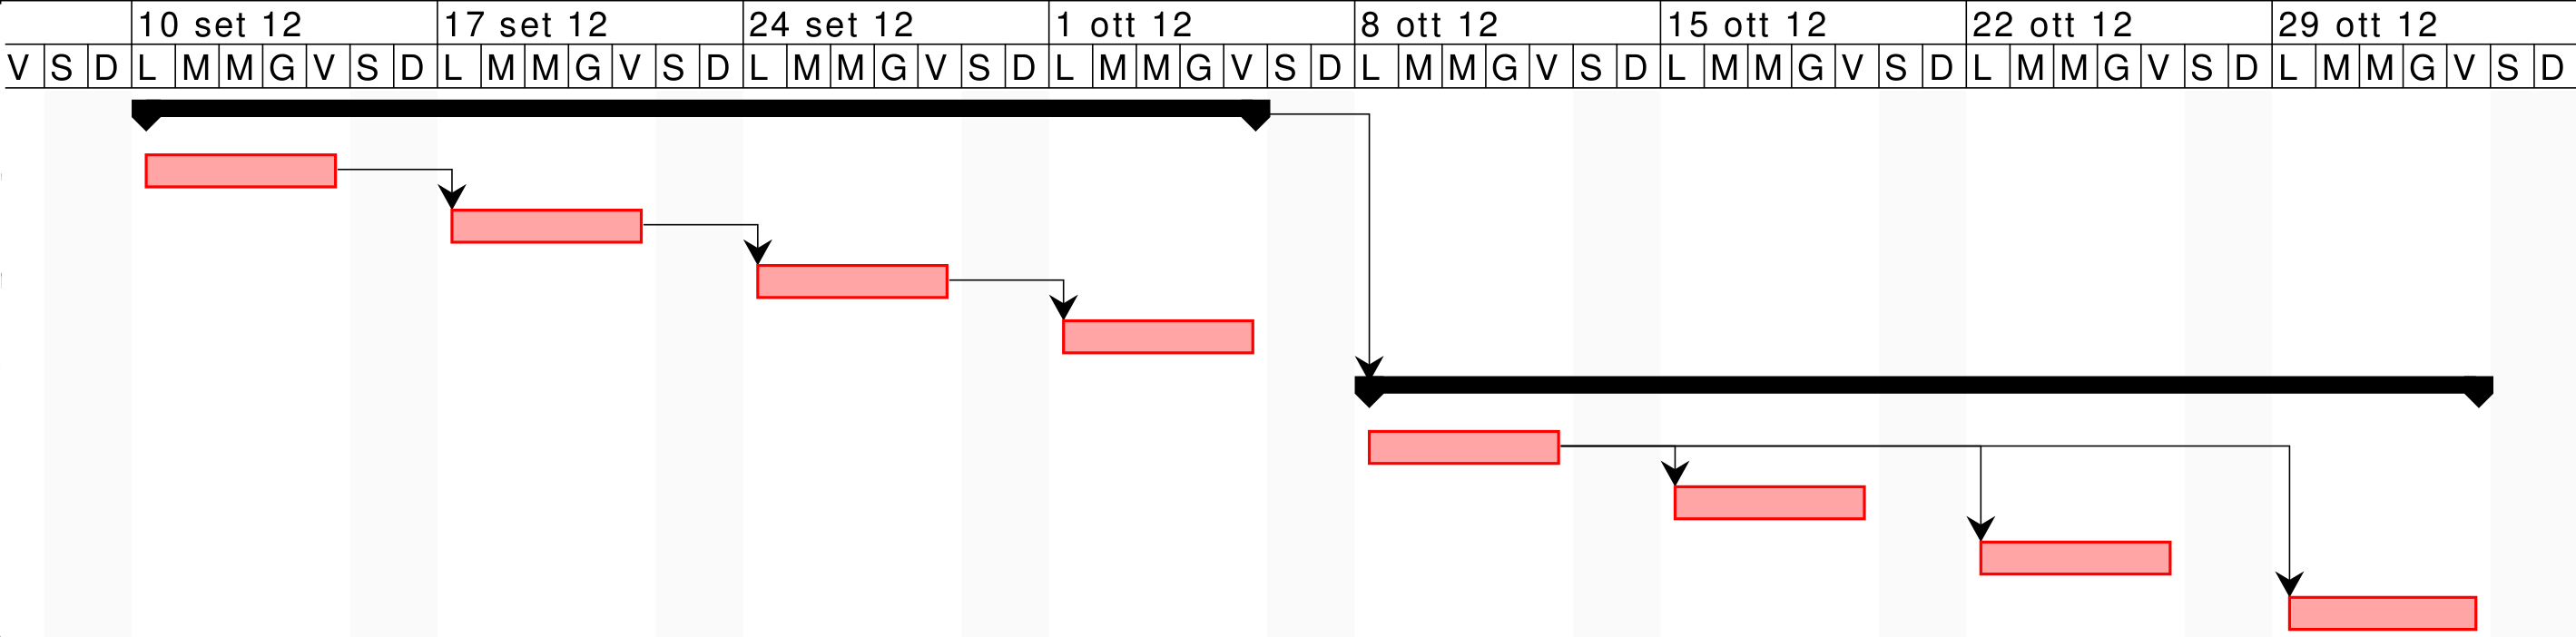
\includegraphics[width=13cm]{img/gantt.png}
		\label{fig:tesi:stage:gantt}
		\caption{Diagramma di Gantt}
	\end{center}
\end{figure}

\section{Norme di stage}
Nel corso dello stage sono stati impiegati diversi strumenti per gestire le attività di progetto e produrre la documentazione prevista.

\begin{table}[ht]
\centering
\begin{tabular}{|l|l|}
\hline
\textsc{Controllo di versione} & \underline{Mercurial} 2.0.2 \\ \hline
\textsc{Editor \LaTeX} & \underline{LaTeXila} 2.4.0 - \underline{gedit} 3.4.0\\ \hline
\textsc{Editor UML} & \underline{UMLet} 11.5.1 \\ \hline
\textsc{Foglio elettronico} & \underline{LibreOffice Calc} 3.6 \\ \hline
\textsc{Gestione database} & \underline{MySQL Workbench} 5.2.42 \\ \hline
\textsc{Mockup} & \underline{Pencil} 2.0.2 \\	\hline
\textsc{Pianificazione} & \underline{ProjectLibre} 1.5.1 \\ \hline
\textsc{Repository} & \underline{Bitbucket} \\ \hline
\textsc{Sistema operativo} & \underline{Ubuntu} 12.04 \\ \hline
\end{tabular}
\caption{Configurazione dell'ambiente di lavoro}
\label{tab:tesi:stage:norme:strumenti}
\end{table}

\paragraph{Documentazione}
La documentazione è redatta in \LaTeX\ e pubblicata in formato \underline{PDF}. A ciascun documento è assegnato un numero di versione $x.y$, ove $x$ rappresenta l'ultima \textsc{versione formale}, rivista e approvata dal referente aziendale e disponibile a terze parti interessate (membri del team di progetto, tutor interno), mentre il numero $y$ si riferisce ad una \textsc{versione preliminare} per uso interno, eventualmente consultabile dal referente aziendale.

\paragraph{Modello relazionale}
Il modello relazionale del database è stato realizzato mediante lo strumento adottato dal team di progetto, ossia l'editor \textit{MySQL Workbench}, per facilitare la condivisione e l'integrazione delle informazioni.

I nomi delle tabelle sono espressi in lingua italiana e contengono solo caratteri alfabetici minuscoli e non accentati, eventualmente separati mediante il simbolo '\textunderscore' (trattino basso). I nomi degli attributi, preceduti dal nome della tabella e dal carattere '.' (punto), sono espressi in lingua italiana e contengono solo caratteri alfabetici in formato \underline{CamelCase}, ove la lettera iniziale è sempre in minuscolo.

\paragraph{Digrammi UML}
Durante l'attività di stage sono stati redatti e inclusi nella documentazione diversi diagrammi \underline{UML} dei casi d'uso, dei package e delle classi, di cui sono presenti svariati esempi nel prosieguo del documento.

I nomi delle sottoclassi riportano - per esteso o in forma abbreviata - l'identificatore della superclasse diretta: nel secondo caso sono presenti - come prefisso - le sole lettere maiuscole, nel medesimo ordine di apparizione.

\paragraph{Casi d'uso}
La notazione utilizzata per identificare un caso d'uso è così definita:
$$UC.x.y$$
ove:
\begin{itemize}
\item $UC$ è l'abbreviazione di \textit{Use Case} (Caso d'uso);
\item $x \in \left\{1,2,\ldots\right\}$ è il numero identificativo del diagramma cui appartiene il caso d'uso;
\item $y \in \left\{1,2,\ldots\right\}$ è il numero associato al caso d'uso.
\end{itemize}

\paragraph{Requisiti funzionali}
I requisiti del sistema software sono univocamente identificati mediante la seguente notazione:
$$Rf.x.y$$
ove:
\begin{itemize}
\item $Rf$ è l'abbreviazione di \textit{requisito funzionale};
\item $x \in \left\{ob,de\right\}$ rappresenta il tipo di requisito funzionale (\textit{ob} per obbligatorio, \textit{de} per desiderabile);
\item $y \in \left\{1,2,\ldots\right\}$ è il numero associato ad un requisito.
\end{itemize}

\paragraph{Tracciamento dei casi d'uso}
Il tracciamento delle dipendenze tra casi d'uso e requisiti software è realizzato mediante un foglio elettronico, ove:
\begin{itemize}
\item ciascuna riga rappresenta un requisito del sistema software;
\item ciascuna colonna rappresenta un caso d'uso;
\item ciascuna cella contiene il carattere 'X' se esiste una relazione di dipendenza tra il caso d'uso e il requisito, altrimenti è vuota.
\end{itemize}

Per ciascuna riga e colonna viene impiegata una semplice formula per asserire la completezza e la necessità della matrice dei requisiti:  
\begin{center}
\texttt{CONTA.SE(A:Z;``X'')}   
\end{center}
ove:
\begin{itemize}
\item \texttt{A:Z} corrisponde all'intervallo di celle di una singola riga o colonna;
\item \texttt{"X"} rappresenta la stringa da cercare;
\item \texttt{CONTA.SE} è una funzione che accetta due argomenti (l'intervallo di celle ed il \textit{pattern}) e restituisce il numero di celle appartenenti all'intervallo contenenti una o più occorrenze del \textit{pattern} specificato.
\end{itemize}

\paragraph{Completezza} Per ogni colonna, se la formula restituisce un valore pari a 0 (zero) sta ad indicare che il requisito utente non è soddisfatto da alcun requisito software.

\paragraph{Necessità} Per ogni riga, se la formula restituisce un valore pari a 0 (zero) sta ad indicare che il requisito software corrispondente è superfluo.

%--------
% SECTION
%--------
\section{Criterio di classificazione}
\label{sec:tesi:stage:criterio-classificazione}
Il patrimonio di conoscenza della piattaforma è garantito essenzialmente dai contenuti pubblicati dagli utenti ed arricchito dal loro valore informativo: ciascuno di essi, a prescindere dalla forma (testo, immagini, audio, video, \ldots) o dalla classe (domanda, discorso, evento, recensione, \ldots), condivide delle informazioni inerenti uno o più elementi del dominio tematico della piattaforma.

\begin{figure}[ht]
\begin{center}
 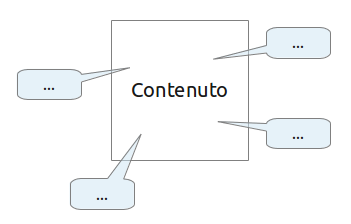
\includegraphics[width=7cm]{img/valore-informativo-contenuto.png}
 \caption{Valore informativo di un contenuto}
 \label{fig:tesi:stage:classificazione:serbatoio-contenuti}
\end{center}
\end{figure}

\subsection{Enciclopedia del sapere}
\label{sec:tesi:stage:criterio-classificazione:enciclopedia}
Attualmente, il limite della piattaforma consiste nell'essere un serbatoio di \textsc{contenuti informativi} disaggregati e priva degli strumenti per classificare e catalogare il sapere custodito conferendovi una struttura ordinata, una sorta di indice in grado di facilitarne la ricerca, il reperimento e la consultazione.

L'obiettivo del criterio di classificazione consiste essenzialmente nel costruire un'enciclopedia del sapere a partire dalle informazioni presenti nei contenuti informativi.

\begin{quotation}
Un'enciclopedia è un'opera letteraria che raccoglie e ordina la sintesi della conoscenza umana in tutti i campi o in un determinato settore. Le enciclopedie sono divise in voci, o lemmi, cui si accede di solito in ordine alfabetico. \cite{wiki:enciclopedia}
\end{quotation}

Il modello concettuale dell'enciclopedia diventa un riferimento utile ad identificare:
\begin{enumerate}
	\item i casi d'uso essenziali concernenti la consultazione del sapere custodito nella piattaforma (ricerca per lemma, argomento o affinità);
	\item gli elementi strutturali del sistema di classificazione (lemmi, accezioni, \ldots);
	\item i requisiti e le specifiche più rilevanti per il criterio di classificazione;
	\item le principali criticità rispetto alla coerenza e consistenza dell'enciclopedia.
\end{enumerate}

\paragraph{Contenuto informativo}
Ciascun contenuto può essere considerato una collezione di frammenti di informazioni (v. figura \ref{fig:tesi:stage:classificazione:serbatoio-contenuti}), che contribuiscono ad arricchire la conoscenza relativa ad uno o più lemmi dell'enciclopedia. Il criterio di classificazione deve quindi tenere traccia della relazione tra contenuti informativi e lemmi per essere in grado di catalogare e ricostruire l'intero sapere disponibile riguardo un certo tema.

\paragraph{Entità}
Nell'ambito della piattaforma, i lemmi vengono definiti entità ($d_i \in D$) e rappresentano elementi concreti (luoghi, persone, eventi, \ldots) o astratti (concetti, temi, \ldots) a cui afferiscono i contenuti.

L'insieme delle entità definite - in un certo istante - all'interno della piattaforma rappresenta il \textsc{dominio della conoscenza} (di seguito per brevità \textsc{dominio}).

\begin{figure}[ht]
	\begin{center}
		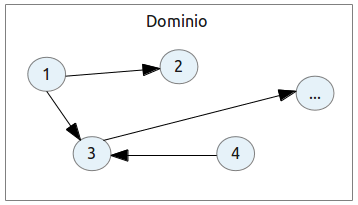
\includegraphics[width=7cm]{img/relazioni-entita.png}
		\label{fig:tesi:stage:fase-uno:entita-relazioni}
		\caption{Relazioni tra le entità del dominio}
	\end{center}
\end{figure}

Così come ciascun lemma di un'enciclopedia contiene spesso riferimenti ad altre voci, che trattano temi specifici o attinenti, nella piattaforma ciascuna entità può riferire o essere riferita da un numero arbitrario di entità distinte e possono esistere riferimenti incrociati, ossia coppie di entità che si citano a vicenda.

Ciò si traduce nel modello relazionale con un vincolo referenziale di tipo molti-a-molti tra le entità, che distingue referenti e riferite e permette di interpretare il dominio $D$ mediante una struttura a grafo orientato ove:
\begin{itemize}
\item ciascun nodo rappresenta un entità;
\item ciascun arco uscente identifica un'\textsc{entità riferita};
\item ciascun arco entrante identifica un'\textsc{entità referente}.
\end{itemize}

\paragraph{Etichette}
Ciascuna entità ha un valore semantico preciso ed univoco, ma dev'essere identificata anche sul piano sintattico mediante un'etichetta ($e_j \in E$), ossia una stringa di lunghezza variabile che consenta agli utenti di riferirla all'interno di ciascun contenuto.

L'insieme di etichette definite in un certo istante costituisce il \textsc{dizionario} della piattaforma.

Il modello illustrato presenta tuttavia due notevoli inconvenienti, che devono essere risolti per soddisfare i requisiti e gli obiettivi fissati: l'ambiguità sintattica e quella semantica.

\subsection{Ambiguità sintattica}
\label{sec:tesi:stage:criterio-classificazione_ambiguità-sintattica}
Nel linguaggio comune, è possibile riferirsi ad una certa entità ($d_i$) con termini o espressioni differenti ($e_{i,j} \in E_i$): la presenza di sinonimi, aventi il medesimo valore semantico ma diversa sintassi, rappresenta un fattore di ambiguità intrinseco e non trascurabile, che trasforma la relazione uno-a-uno tra entità ed etichette in una di tipo uno-a-molti.

\begin{figure}[ht]
	\begin{center}
		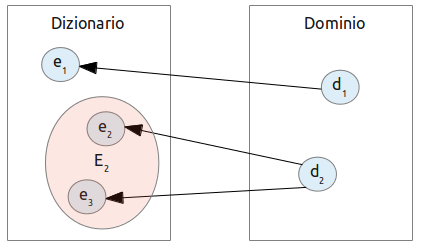
\includegraphics[width=7cm]{img/ambiguita-sintattica.png}
		\label{fig:tesi:stage:fase-uno:ambiguita-sintattica}
		\caption{Ambiguità sintattica di un'entità}
	\end{center}
\end{figure}

Il criterio di classificazione è dunque chiamato a conciliare la possibilità per l'utente di riferirsi ad una certa entità con etichette differenti e l'esigenza di identificarla univocamente nei contenuti informativi.

\paragraph{Sinonimi}
La gestione dei sinonimi di un'entità rappresenta un aspetto cruciale, poiché scegliere tra i possibili sinonimi un'etichetta arbitraria con cui identificare un'entità ed ignorare i rimanenti, pur semplificando il modello, costringerebbe gli utenti a conoscere e ad utilizzare solo quell'etichetta, imponendo una scelta del tutto arbitraria e - in quanto tale - fortemente soggettiva.

Per facilitare la ricerca di un'entità è opportuno includere e conservare nel dizionario tutte le etichette note o utilizzate dagli utenti, così da rendere il sistema sempre più accurato nell'individuare e riconoscere l'entità cui un utente fa riferimento ogni qualvolta utilizza una certa etichetta. Con il passare del tempo, il numero dei sinonimi di ciascuna entità è destinato a crescere grazie al contributo degli utenti, garantendo così una migliore copertura sintattica.

La proliferazione di sinonimi, ossia etichette equivalenti sul piano semantico ma sintatticamente differenti, rischia tuttavia di avere pesanti ripercussioni sull'efficacia del criterio di classificazione e particolarmente sull'efficienza della ricerca: se ai contenuti vengono assegnate delle etichette, reperire tutte e sole le informazioni inerenti una certa entità richiederebbe infatti di cercare riscontri nei contenuti pubblicati per ogni etichetta con cui possa venir riferita.

\paragraph{Contenuti}
A tale inconveniente si pone rimedio facilmente definendo una relazione molti-a-molti tra le entità e i contenuti, che ignori le etichette utilizzate per indicarle.

Così facendo si preserva l'identificazione univoca di ciascuna entità nei contenuti informativi, almeno sul piano semantico, e si guadagna in termini di efficienza.

Si considerino il dizionario $E$ ed il dominio $D$. Il numero medio $\alpha$ di etichette associate a ciascuna entità risulta pari a:\footnote{Poiché la relazione tra etichette ed entità è di tipo uno-a-molti, ciascuna etichetta è associata ad una ed una sola entità. Ne consegue che $P = \{ E_0, E_1, \ldots \}$ è una partizione di $E$, ossia vale $\bigcup E_i = E$ e $\forall A \in P, B \in P: A \neq B \implies A \cap B = \emptyset$.}
\begin{equation} \label{eq:tesi:stage:etichette-per-entità}
\alpha = \frac{\left|E_0\right| + \left|E_1\right| + \ldots}{\left|D\right|} = \frac{\sum{\left|E_i\right|}}{\left|D\right|}
\end{equation}
ove
\begin{equation} \label{eq:tesi:stage:dizionario}
\sum{\left|E_i\right|} = \left|E\right|
\end{equation}

Ciò significa intuitivamente che assegnare ai contenuti un'etichetta arbitraria aumenterebbe di una costante moltiplicativa $\alpha$ la complessità dell'operazione di ricerca, che dovrebbe essere ripetuta per ciascuna delle $\alpha$ etichette anziché per la sola entità corrispondente.\footnote{Si assuma per semplicità che la ricerca verifichi - per ciascun contenuto - quali entità o etichette cercate siano presenti, una per volta, e che la complessità computazionale sia equivalente in entrambi i casi.}

\paragraph{Etichette}
Tuttavia, per riferire un'entità nella piattaforma web occorre caratterizzarla anche sul piano sintattico. Sebbene non vi siano particolari controindicazioni nel permettere all'utente di scegliere l'etichetta da utilizzare nei contenuti pubblicati, si rischia di:
\begin{itemize}
	\item generare ambiguità e confusione tra gli utenti stessi, rendendo poco intuitivo stabilire se due entità citate in due contenuti diversi e con etichette differenti rappresentino effettivamente la stessa;
	\item dover aggiungere alla relazione tra entità e contenuti un'informazione aggiuntiva, ossia l'etichetta scelta per indicarla.
\end{itemize}

Per tale ragione, si individua arbitrariamente - per ciascuna entità $d_i$ - un'\textsc{etichetta primaria} ($e_{i,0} \in E_i$), che la identifica univocamente nell'ambito della piattaforma, mentre le restanti (\textsc{etichette secondarie}) ne vengono considerate sinonimi.

Così facendo si introducono tuttavia alcuni vincoli aggiuntivi sulla relazione, che risulta scissa in due distinte:
\begin{enumerate}
	\item una relazione di tipo uno-a-uno tra l'entità e la corrispondente etichetta primaria;
	\item una relazione uno-a-molti tra l'entità e le etichette secondarie.
\end{enumerate}

\begin{figure}[ht]
	\begin{center}
		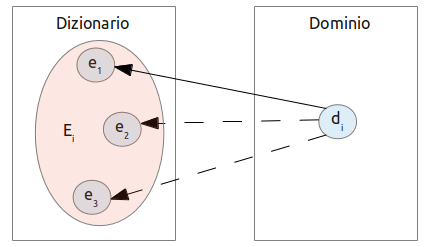
\includegraphics[width=7cm]{img/etichette-primarie-secondarie.png}
		\label{fig:tesi:stage:fase-uno:entita-sintassi-semantica}
		\caption{Etichetta primaria e secondarie}
	\end{center}
\end{figure}

In conclusione, il nodo cruciale della soluzione individuata consiste nel mantenere separato l'aspetto semantico (le entità) da quello sintattico (le etichette): ogni qualvolta l'utente ricerca o assegna un'etichetta ad un contenuto, il sistema traduce il suo ingresso sintattico (l'etichetta) in un'uscita semantica (l'entità corrispondente).

Tale meccanismo è tuttavia soggetto ad alcune complicazioni, dovute all'ambiguità semantica di ciascuna etichetta.

\subsection{Ambiguità semantica}
\label{sec:tesi:stage:criterio-classificazione:ambiguità-semantica}
Riprendendo il modello dell'enciclopedia, si osserva come ciascuna etichetta $e_j$ possa avere svariate \textsc{accezioni} ($a_{j,k} \in A_j$), ciascuna delle quali ne individua un significato differente e si riferisce ad un'entità distinta.

\begin{figure}[ht]
	\begin{center}
		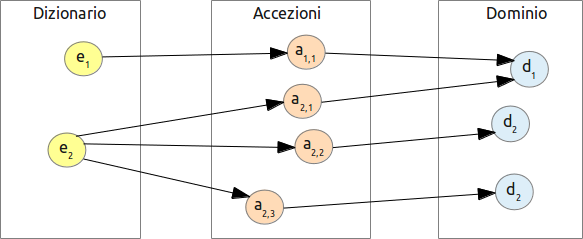
\includegraphics[width=10.5cm]{img/ambiguita-semantica.png}
		\caption{Accezioni di un'etichetta}
		\label{fig:tesi:stage:fase-uno:etichette-accezioni}
	\end{center}
\end{figure}

Sebbene la natura tematica della piattaforma tenda a mitigare la presenza di etichette aventi accezioni multiple, tale eventualità non può essere esclusa e dev'essere dunque opportunamente gestita.

Occorre innanzi tutto rivedere la relazione uno-a-molti tra entità ed etichette, che diventa di tipo molti-a-molti e per cui vale la proprietà illustrata di seguito.

Siano $a_{j,k}$ e $a_{j,k'}$ accezioni distinte di un'etichetta $e_j$ e sia definita la funzione
\begin{equation}
f(a_{j,k}): A_j \rightarrow D
\end{equation}
che restituisce l'entità $d_i$ riferita dall'accezione $a_{j,k}$. Allora
\begin{equation}
a_{j,k} \neq a_{j,k'} \implies f(a_{j,k}) \neq f(a_{j,k'})
\end{equation}

\begin{figure}[ht]
	\begin{center}
		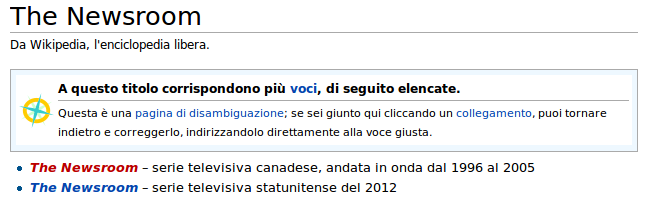
\includegraphics[width=12cm]{img/disambigua.png}
		\label{fig:tesi:stage:classificazione:disambiguazione}
		\caption{Pagina di disambiguazione \cite{wiki:disambigua}}
	\end{center}
\end{figure}

L'equazione \ref{eq:tesi:stage:etichette-per-entità} conserva la propria validità, mentre la \ref{eq:tesi:stage:dizionario} dev'essere modificata per riflettere la differente molteplicità della suddetta relazione, ossia che ciascuna etichetta riferisce una o più entità:
\begin{equation}
	\sum{\left|E_i\right|} = \sum{\left|B_i\right|} = \left|A\right| =	\sum{\left|A_j\right|} \geq \left|E\right|
\end{equation}

%La prima uguaglianza esprime una banale identità tra le etichette di un'entità e  e le accezioni corrispondenti; la seconda discende dal fatto che $P' = {B_1,B_2,\ldots}$ rappresenta una partizione di $A$ rispetto alle entità, mentre la successiva uguaglianza si deduce analogamente dal fatto che $P''={A_1, A_2, \ldots}$ è anch'essa partizione di $A$ (rispetto alle etichette); l'ultima disuguaglianza si deduce osservando che $\forall j \left|A_j\right| \geq 1$, ossia per ciascuna etichetta del dizionario esiste almeno un'accezione.

A ciascuna entità continuano ad essere associate una e una sola etichetta primaria e un numero arbitrario (anche nullo) di etichette secondarie. Ove ciascuna etichetta può riferirsi a diverse entità, tale distinzione varia a seconda dell'accezione considerata, poiché la medesima etichetta può essere primaria rispetto ad un entità e secondaria rispetto ad un'altra.

Per preservare i suddetti vincoli sulle relazioni tra etichette ed entità, si classificano le accezioni in \textsc{chiave} ($a_{j,0}$) o \textsc{sinonimiche} ($a_{j,1},\ldots$), a seconda che l'etichetta risulti rispettivamente primaria o secondaria per l'entità corrispondente. In questo modo si riesce a trasferire tale distinzione dalle etichette alle accezioni, preservando la percezione della relazione dal punto di vista dell'entità.

\begin{figure}[ht]
	\begin{center}
		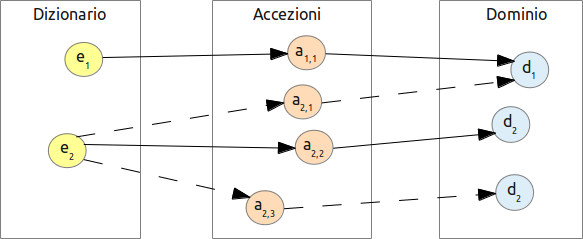
\includegraphics[width=10.5cm]{img/accezioni-chiave-sinonimiche.png}
		\caption{Accezioni chiave e sinonimiche}
		\label{fig:tesi:stage:fase-uno:accezioni-chiave-sinonimiche}
	\end{center}
\end{figure}

A risentire maggiormente dell'esistenza delle accezioni è il processo di ricerca di un'entità $d_i$ a partire da un'etichetta $e_j$: se $\left|A_j\right|\geq 2$ l'identificazione dell'entità richiede - da parte dell'utente - la selezione di un'accezione $a_{j,k} \in A_j$ tra le $\left|A_j\right|$ disponibili per indicare esplicitamente l'entità cui fa riferimento.

\subsection{Modello relazionale}

\begin{figure}[ht]
	\begin{center}
		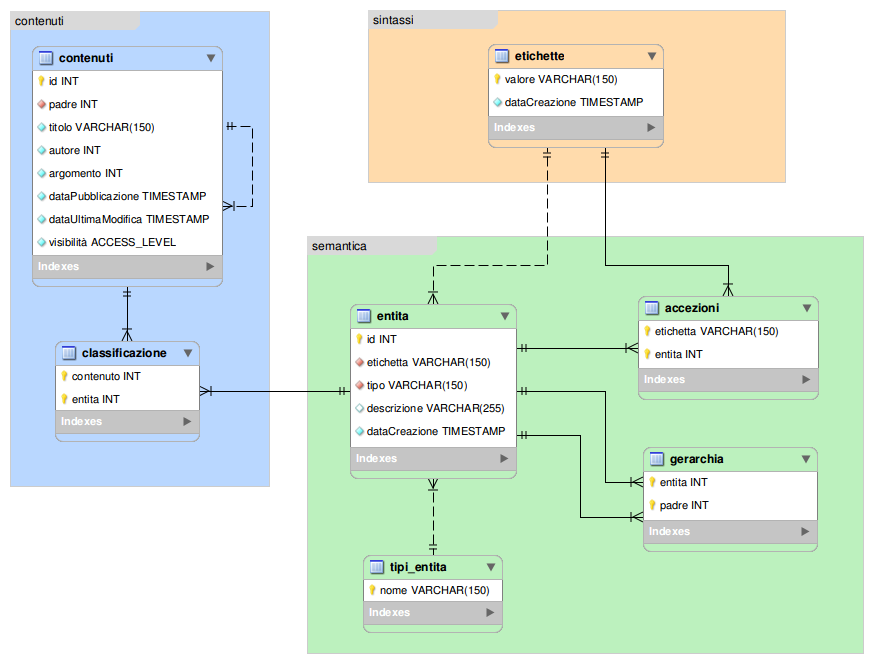
\includegraphics[width=12cm]{img/modello-er.png}
		\caption[Modello relazionale]{Modello relazionale del criterio di classificazione}
		\label{fig:tesi:stage:er:modello}
	\end{center}
\end{figure}

Al termine della fase progettuale, si rende necessario modificare il modello relazionale della piattaforma per integrare le informazioni addizionali legate al nuovo criterio di classificazione.

Rispetto all'immagine \ref{fig:tesi:stage:er:modello}, la sola tabella \textsf{contenuti} risulta importata dal modello relazionale della piattaforma per evidenziare alcuni vincoli fondamentali. Le rimanenti sono organizzate in tre \textit{layer} (\textsf{contenuti}, \textsf{semantica} e \textsf{sintassi}) per chiarirne il ruolo all'interno del sistema di classificazione.

\paragraph{Etichette}
Le etichette sono rappresentate mediante la tabella \textsf{etichette} e sono identificate univocamente dalla stringa associata, che rappresenta l'attributo \textsf{etichette.valore}. Tale scelta risponde alla naturale identificazione dell'etichetta nella sequenza di caratteri corrispondente, costituisce una garanzia contro la presenza di duplicati e consente di recuperare il valore dell'etichetta primaria di un'entità senza dover effettuare un'operazione di \textit{join} tra le tabelle \textsf{entita} ed \textsf{etichette}.

\paragraph{Accezioni}
Le accezioni rappresentano un legame univoco tra le etichette e le entità e possono essere di tipo chiave o sinonimico. Esse non presentano attributi propri significativi, ma prevedono tre vincoli referenziali:
\begin{enumerate}
\item a ciascuna entità è associata una e una sola accezione chiave (relazione uno-a-uno), che ne identifica l'etichetta primaria;
\item a ciascuna entità sono associate $0\ldots n$ accezioni sinonimiche (relazione uno-a-molti), che rappresentano i sinonimi dell'etichetta primaria;
\item ciascuna etichetta possiede $0\ldots n$ accezioni (relazione uno-a-molti).
\end{enumerate}

\begin{figure}[ht]
	\begin{center}
		
\includegraphics{img/placeholder.png}
		\caption{Modello ad oggetti delle accezioni}
		\label{fig:tesi:stage:er:accezioni}
	\end{center}
\end{figure}

Ne consegue che sia la superclasse (\textsf{accezioni}) sia le sottoclassi \linebreak(\textsf{accezioni\textunderscore chiave} e \textsf{accezioni\textunderscore sinonimiche}) presentano dei vincoli referenziali; in particolare, la presenza delle prime due relazioni costringe a distinguere - dal punto di vista dell'entità - tra accezioni chiave e sinonimiche.

Per modellare tale scenario vengono presi in considerazione tre possibili approcci:
\begin{description}
\item[Tabella unica] \hfill \\
La tabella unica ben si adatta a gestire l'assenza di attributi propri per le sottoclassi e ad esprimere i vincoli referenziali che coinvolgono la superclasse, ma non è in grado di esprimere e adeguatamente rappresentare quelli coinvolgenti le sottoclassi.
\item[Partizionamento orizzontale] \hfill \\
Il partizionamento orizzontale riesce a modellare i vincoli referenziali delle sottoclassi, ma non quello della superclasse, e genera due classi aventi i medesimi attributi.
\item[Partizionamento verticale] \hfill \\
Il partizionamento verticale consente di modellare correttamente tutti e tre i vincoli referenziali, relativi sia alla superclasse sia alle sottoclassi. Tuttavia si rende più complesso modificare il tipo di un'accezione e si introduce l'esigenza di un'operazione \textit{join} per recuperare la lista completa delle accezioni, pur non possedendo le sottoclassi attributi propri.
\end{description}

\pagebreak
A seguito di alcune osservazioni si decide di adottare la soluzione della tabella unica:
\begin{itemize}
\item la distinzione tra etichette chiave e sinonimiche ha rilevanza essenzialmente dal punto di vista della classe \textsf{entita};
\item il vincolo referenziale tra \textsf{etichette} ed \textsf{accezioni} suggerisce che la distinzione di cui al punto precedente sia irrilevante dal punto di vista delle etichette, ragion per cui risulta utile mantenere tutte le accezioni nella medesima tabella.\footnote{Si consideri ad esempio il caso d'uso della ricerca di un'entità a partire da un'etichetta, ove occorre recuperare la lista completa delle relative accezioni.}
\item le sottoclassi non hanno attributi propri, per cui il partizionamento verticale e orizzontale sono ritenute soluzioni inadeguate.
\end{itemize}

Il soddisfacimento delle condizioni richieste viene raggiunto eliminando qualsiasi riferimento al tipo dell'accezione nella classe \textsf{accezioni} e modellando direttamente la relazione uno-a-uno tra le entità e le relative etichette primarie mediante un vincolo referenziale di chiave esterna nella classe \textsf{entita} (\textsf{entita.etichetta}), che identifica la corrispondente etichetta primaria (\textsf{etichette.valore}). Così facendo si riescono ad esprimere tutti i vincoli referenziali senza la necessità di definire le sottoclassi.
